\documentclass{article}
\usepackage[utf8]{inputenc}
\usepackage{tikz}
\usetikzlibrary{shapes.geometric, arrows}

\tikzstyle{startstop} = [rectangle, rounded corners, text width = 3cm, minimum width=3cm, minimum height=1cm,text centered, draw=black, fill=red!30]

\tikzstyle{io} = [trapezium, trapezium left angle=70, trapezium right angle=110, minimum width=3cm, minimum height=1cm, text width = 3cm, text centered, draw=black, fill=blue!30]

\tikzstyle{process} = [rectangle, minimum width = 3cm,
minimum height = 1cm, text centered, text width = 3cm, draw = black, fill = orange!30]

\tikzstyle{decision} = [ellipse, minimum width = 3cm,
minimum height = 1cm, text centered, draw = black, fill =green!30]

\tikzstyle{arrow} = [thick, -> , >=stealth]

\begin{document}
\begin{centering}
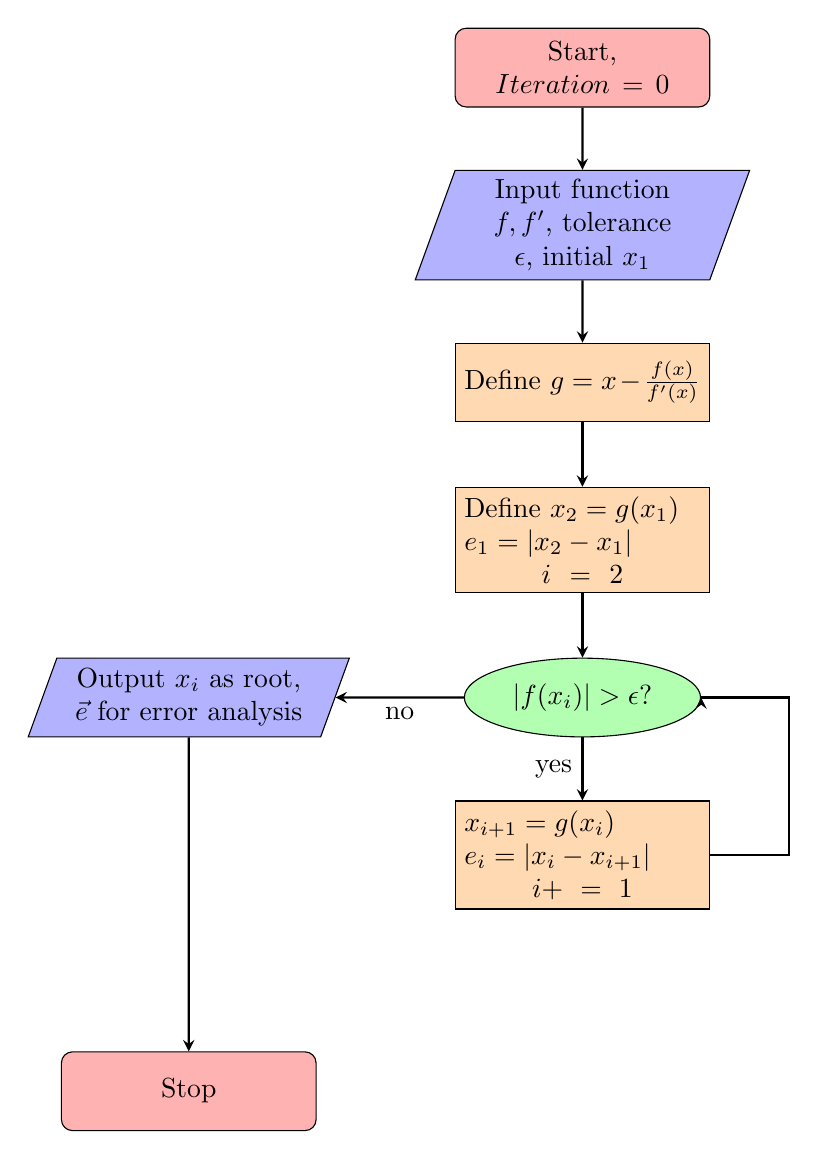
\begin{tikzpicture}[node distance = 2cm]

    
\node (start) [startstop] {Start, $Iteration = 0$};
\node (in1) [io, below of=start] {Input function $f, f'$, tolerance $\epsilon$, initial $x_1$};
\node (pro1) [process, below of=in1] {Define $g = x - \frac{f(x)}{f'(x)}$};
\node (pro2) [process, below of=pro1] {Define $x_2 = g(x_1)\newline e_1 = |x_2-x_1|\newline i=2$};
\node (dec1) [decision, below of=pro2] {$|f(x_i)| > \epsilon$?};
\node (pro3) [process, below of=dec1] {$x_{i+1} = g(x_i)\newline e_i = |x_i - x_{i+1}|\newline i += 1$};

\node (out1) [io, left of =dec1, xshift = -3cm] {Output $x_i$ as root, $\vec{e}$ for error analysis};

\node (stop) [startstop, below of= out1, yshift = -3cm] {Stop};

%% arrows
\draw [arrow] (start) -- (in1);
\draw [arrow] (in1) -- (pro1);
\draw [arrow] (pro1) -- (pro2);
\draw [arrow] (pro2) -- (dec1);
\draw [arrow] (dec1) -- node[anchor = north]{no}(out1);
\draw [arrow] (dec1) -- node[anchor = east]{yes}(pro3);

%\draw [arrow]  (pro3.west) |- ([shift={(-5.5cm,0mm)}]pro3.west) |- ([shift={(-5cm,0mm)}]dec2.west) -| (dec2.west);
\draw [arrow]  (pro3.east) -- + (1,0) -- +(1,2) -| (dec1.east);
%\draw [arrow] (dec1.east) -- + (1,0) |- (pro3b)
\draw [arrow]  (out1) -- (stop);

\end{tikzpicture}

\end{centering}

\end{document}